% Options for packages loaded elsewhere
\PassOptionsToPackage{unicode}{hyperref}
\PassOptionsToPackage{hyphens}{url}
%
\documentclass[
]{article}
\usepackage{amsmath,amssymb}
\usepackage{iftex}
\ifPDFTeX
  \usepackage[T1]{fontenc}
  \usepackage[utf8]{inputenc}
  \usepackage{textcomp} % provide euro and other symbols
\else % if luatex or xetex
  \usepackage{unicode-math} % this also loads fontspec
  \defaultfontfeatures{Scale=MatchLowercase}
  \defaultfontfeatures[\rmfamily]{Ligatures=TeX,Scale=1}
\fi
\usepackage{lmodern}
\ifPDFTeX\else
  % xetex/luatex font selection
\fi
% Use upquote if available, for straight quotes in verbatim environments
\IfFileExists{upquote.sty}{\usepackage{upquote}}{}
\IfFileExists{microtype.sty}{% use microtype if available
  \usepackage[]{microtype}
  \UseMicrotypeSet[protrusion]{basicmath} % disable protrusion for tt fonts
}{}
\makeatletter
\@ifundefined{KOMAClassName}{% if non-KOMA class
  \IfFileExists{parskip.sty}{%
    \usepackage{parskip}
  }{% else
    \setlength{\parindent}{0pt}
    \setlength{\parskip}{6pt plus 2pt minus 1pt}}
}{% if KOMA class
  \KOMAoptions{parskip=half}}
\makeatother
\usepackage{xcolor}
\usepackage[margin=1in]{geometry}
\usepackage{longtable,booktabs,array}
\usepackage{calc} % for calculating minipage widths
% Correct order of tables after \paragraph or \subparagraph
\usepackage{etoolbox}
\makeatletter
\patchcmd\longtable{\par}{\if@noskipsec\mbox{}\fi\par}{}{}
\makeatother
% Allow footnotes in longtable head/foot
\IfFileExists{footnotehyper.sty}{\usepackage{footnotehyper}}{\usepackage{footnote}}
\makesavenoteenv{longtable}
\usepackage{graphicx}
\makeatletter
\def\maxwidth{\ifdim\Gin@nat@width>\linewidth\linewidth\else\Gin@nat@width\fi}
\def\maxheight{\ifdim\Gin@nat@height>\textheight\textheight\else\Gin@nat@height\fi}
\makeatother
% Scale images if necessary, so that they will not overflow the page
% margins by default, and it is still possible to overwrite the defaults
% using explicit options in \includegraphics[width, height, ...]{}
\setkeys{Gin}{width=\maxwidth,height=\maxheight,keepaspectratio}
% Set default figure placement to htbp
\makeatletter
\def\fps@figure{htbp}
\makeatother
\setlength{\emergencystretch}{3em} % prevent overfull lines
\providecommand{\tightlist}{%
  \setlength{\itemsep}{0pt}\setlength{\parskip}{0pt}}
\setcounter{secnumdepth}{-\maxdimen} % remove section numbering
\ifLuaTeX
  \usepackage{selnolig}  % disable illegal ligatures
\fi
\IfFileExists{bookmark.sty}{\usepackage{bookmark}}{\usepackage{hyperref}}
\IfFileExists{xurl.sty}{\usepackage{xurl}}{} % add URL line breaks if available
\urlstyle{same}
\hypersetup{
  hidelinks,
  pdfcreator={LaTeX via pandoc}}

\author{}
\date{\vspace{-2.5em}}

\begin{document}

\emph{Author: Lennart Marx}

\emph{Supervisor: Henri Funk}

\emph{Degree: Master}

\hypertarget{sm}{%
\section{Statistical streamflow modelling}\label{sm}}

\hypertarget{abstract}{%
\subsection{Abstract}\label{abstract}}

This study evaluates and compares the performance of Long Short-Term
Memory (LSTM) networks and Temporal Fusion Transformers (TFT) in
forecasting streamflows up to seven days ahead, using historical
streamflow data alongside precipitation and temperature as covariates.
Data from the Regen River in Bavaria, Germany, was used. Preprocessing
involved spatial averaging of meteorological data within defined
catchments. Results indicate that while both models face challenges in
predicting extreme values, TFT maintains more consistent accuracy over
longer forecast horizons while pure LSTM model's predictions decline
sharply in performance with increasing lead time. The study highlights
the importance of future known meteorological variables in achieving
accurate predictions and suggests avenues for future research to enhance
model robustness and data preprocessing techniques.

\hypertarget{introduction}{%
\subsection{Introduction}\label{introduction}}

Accurate streamflow prediction is beneficial for a variety of
applications, including flood forecasting or hydroelectric power
generation. Timely and precise flood predictions can mitigate the impact
of flood events, protecting lives and property. Similarly, reliable
streamflow forecasts are essential for optimizing the operation of
hydroelectric plants, ensuring efficient energy production and
contributing to the stability of power grids.

Streamflow refers to the flow of water in rivers and streams,
originating from precipitation, melting snow, and groundwater discharge.
It is typically measured in cubic meters per second (m³/s).

In recent years, machine learning techniques have emerged as powerful
tools for forecasting in various domains, including hydrology.
Traditional hydrological models often rely on extensive datasets and
intricate physical parameters, which can be challenging to obtain and
process. In contrast, machine learning models such as Long Short-Term
Memory (LSTM) networks offer an alternative approach by learning
patterns directly from historical data. These models have shown promise
in capturing the complex, nonlinear relationships inherent in
hydrological systems.

This study aims to evaluate and compare the performance of LSTM and TFT
models in forecasting streamflows up to seven days ahead. By
incorporating precipitation and temperature as future known covariates
alongside historical streamflow data, we seek to determine the
effectiveness of these models in predicting streamflows.

Understanding the strengths and limitations of these models is essential
for their practical application. Flood events often involve extreme
values that can be difficult to predict accurately, while hydroelectric
generation requires consistent and reliable forecasts over varying time
horizons. Thus, this research not only assesses the overall accuracy of
LSTM and TFT models but also examines their performance in predicting
extreme streamflow values and their resource dependency, providing
insights into their feasibility for real-world applications.

\hypertarget{data}{%
\subsection{Data}\label{data}}

\hypertarget{preperation}{%
\subsubsection{Preperation}\label{preperation}}

The streamflow data is gathered from the bavarian hydrology authority
(GKD). They provide freely accessible data on most water bodies in
Bavaria.Focusing on rivers of medium size where the entire length is
flowing inside of the area of the state of Bavaria, the river Regen
located north/east of the city of Regensburg was chosen as a bases for
this study.The GKD posesses 21 streamflow gauging stations located at
the Regen or any of its tributary rivers. For the Regen river, data
between 2014 and 2024 was available with daily measurements on the
streamflows including the coordinates of the the gauging station. This
study focused on the 15207507 Marienthal gauging station that was
located closest to the final outflow towards the Danube river. Utilizing
the HydroRIVERS dataset, which contains the shapes of rivers all over
the world, it was possible the acquire the shape of the Regen along with
its geolocation as shown in figure @ref(fig:1).

\begin{figure}

{\centering \includegraphics[width=0.8\linewidth]{work/07-hydroLSTM/images/regen_stations} 

}

\caption{Streamflow Gauging Stations that provide there measurements at the GKD along the Regen river}\label{fig:1}
\end{figure}

A catchment also known as a drainage basin or watershed, is an area of
land where all precipitation collects and drains off into a common
outlet, such as a river, bay, or other body of water. The boundaries of
a catchment are defined by the highest points of land around the
drainage area, often referred to as the drainage divide. These catchment
areas will later be used to determine the variables for precipitation
that are used to forecast the streamflows of the river. Taking advantage
of the HydroBASINS dataset, that contains the shapes of basins all over
the world in different resolutions. With the software QGIS a
Geoinformation System (GIS) all basins were chosen that completely
contain the river Regen Shape, which led to the 19 defined chatchments
that can be seen figure @ref(fig:2).

\begin{figure}

{\centering \includegraphics[width=500]{work/07-hydroLSTM/images/river_catch} 

}

\caption{Catchments defined for the Regen river based on the HydroBASINS shapefile dataset}\label{fig:2}
\end{figure}

The ERA5 reanalysis Dataset published by the copernicus project,
contains a plethora of meteorological Data in the form of rasterized
Data. Each data cell contains information of when it occured,where it
occured in the form of longitude and latitude coordinates as well as the
information on a meteorological variables. As suggested in (PAPER
SOURCE), for this study the variables 2 meter temperature and total
precipitation were selected in the area of the Regen and for the past 10
years.

\hypertarget{preprocessing}{%
\subsubsection{Preprocessing}\label{preprocessing}}

The measuring station 15207507 contained 1 missing value which was
imputed by linear interpolation. As suggested in (PAPER Source) non
centered moving average smoothing with a window size of 3 was applied to
the streamflow data as can be seen in figure @ref(fig:3).

\begin{figure}

{\centering 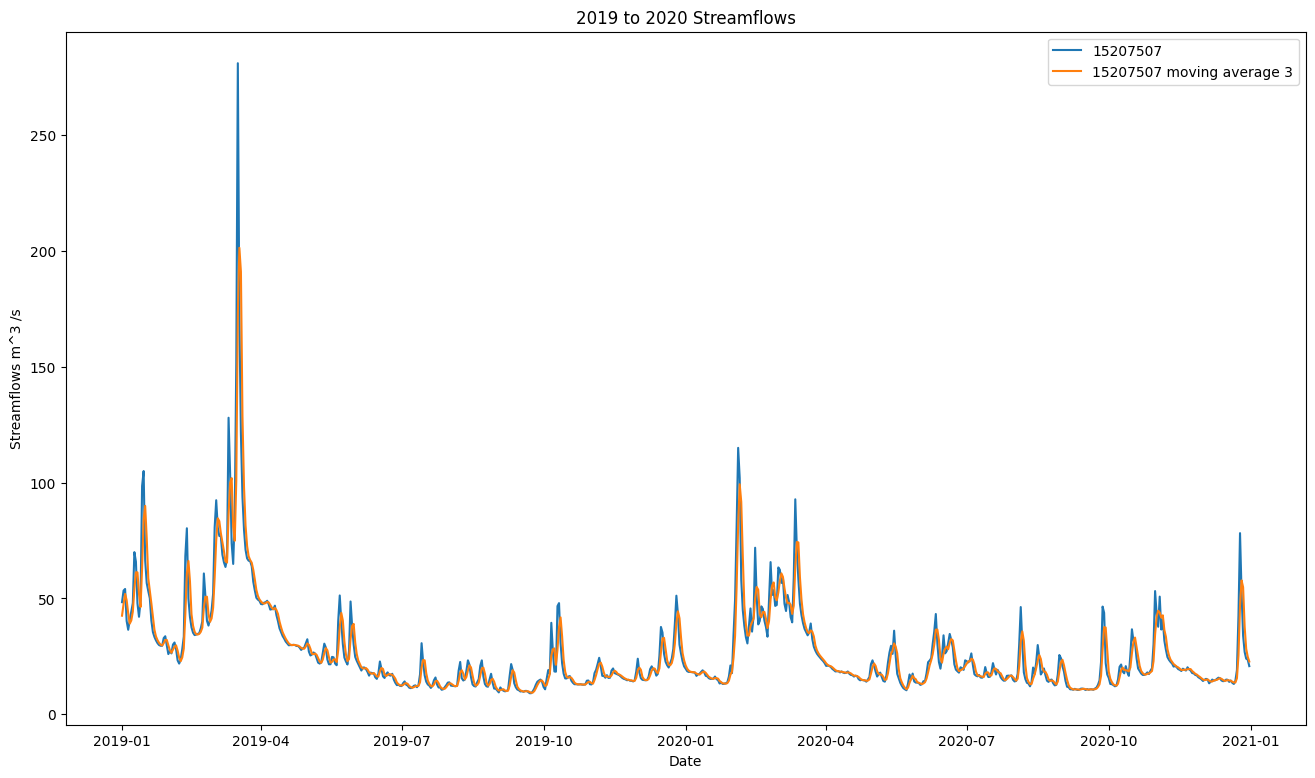
\includegraphics[width=500]{work/07-hydroLSTM/images/Moving_Average} 

}

\caption{streamflows of the 15207507 Marienthal gauging stations before and after applying moving average smoothing}\label{fig:3}
\end{figure}

To combine the rasterized meteorological data from ERA5 with the
streamflows of the Regen, it is necessary to only take precipitation
into account that occurs within the defined catchments. To achieve this,
a weighted average is calculated, where the weights are determined by
the area size of the intersection between the raster cell of the
meteorological data and the catchment. This can be seen in a schematic
visualization in figure @ref(fig:4).

\begin{figure}

{\centering 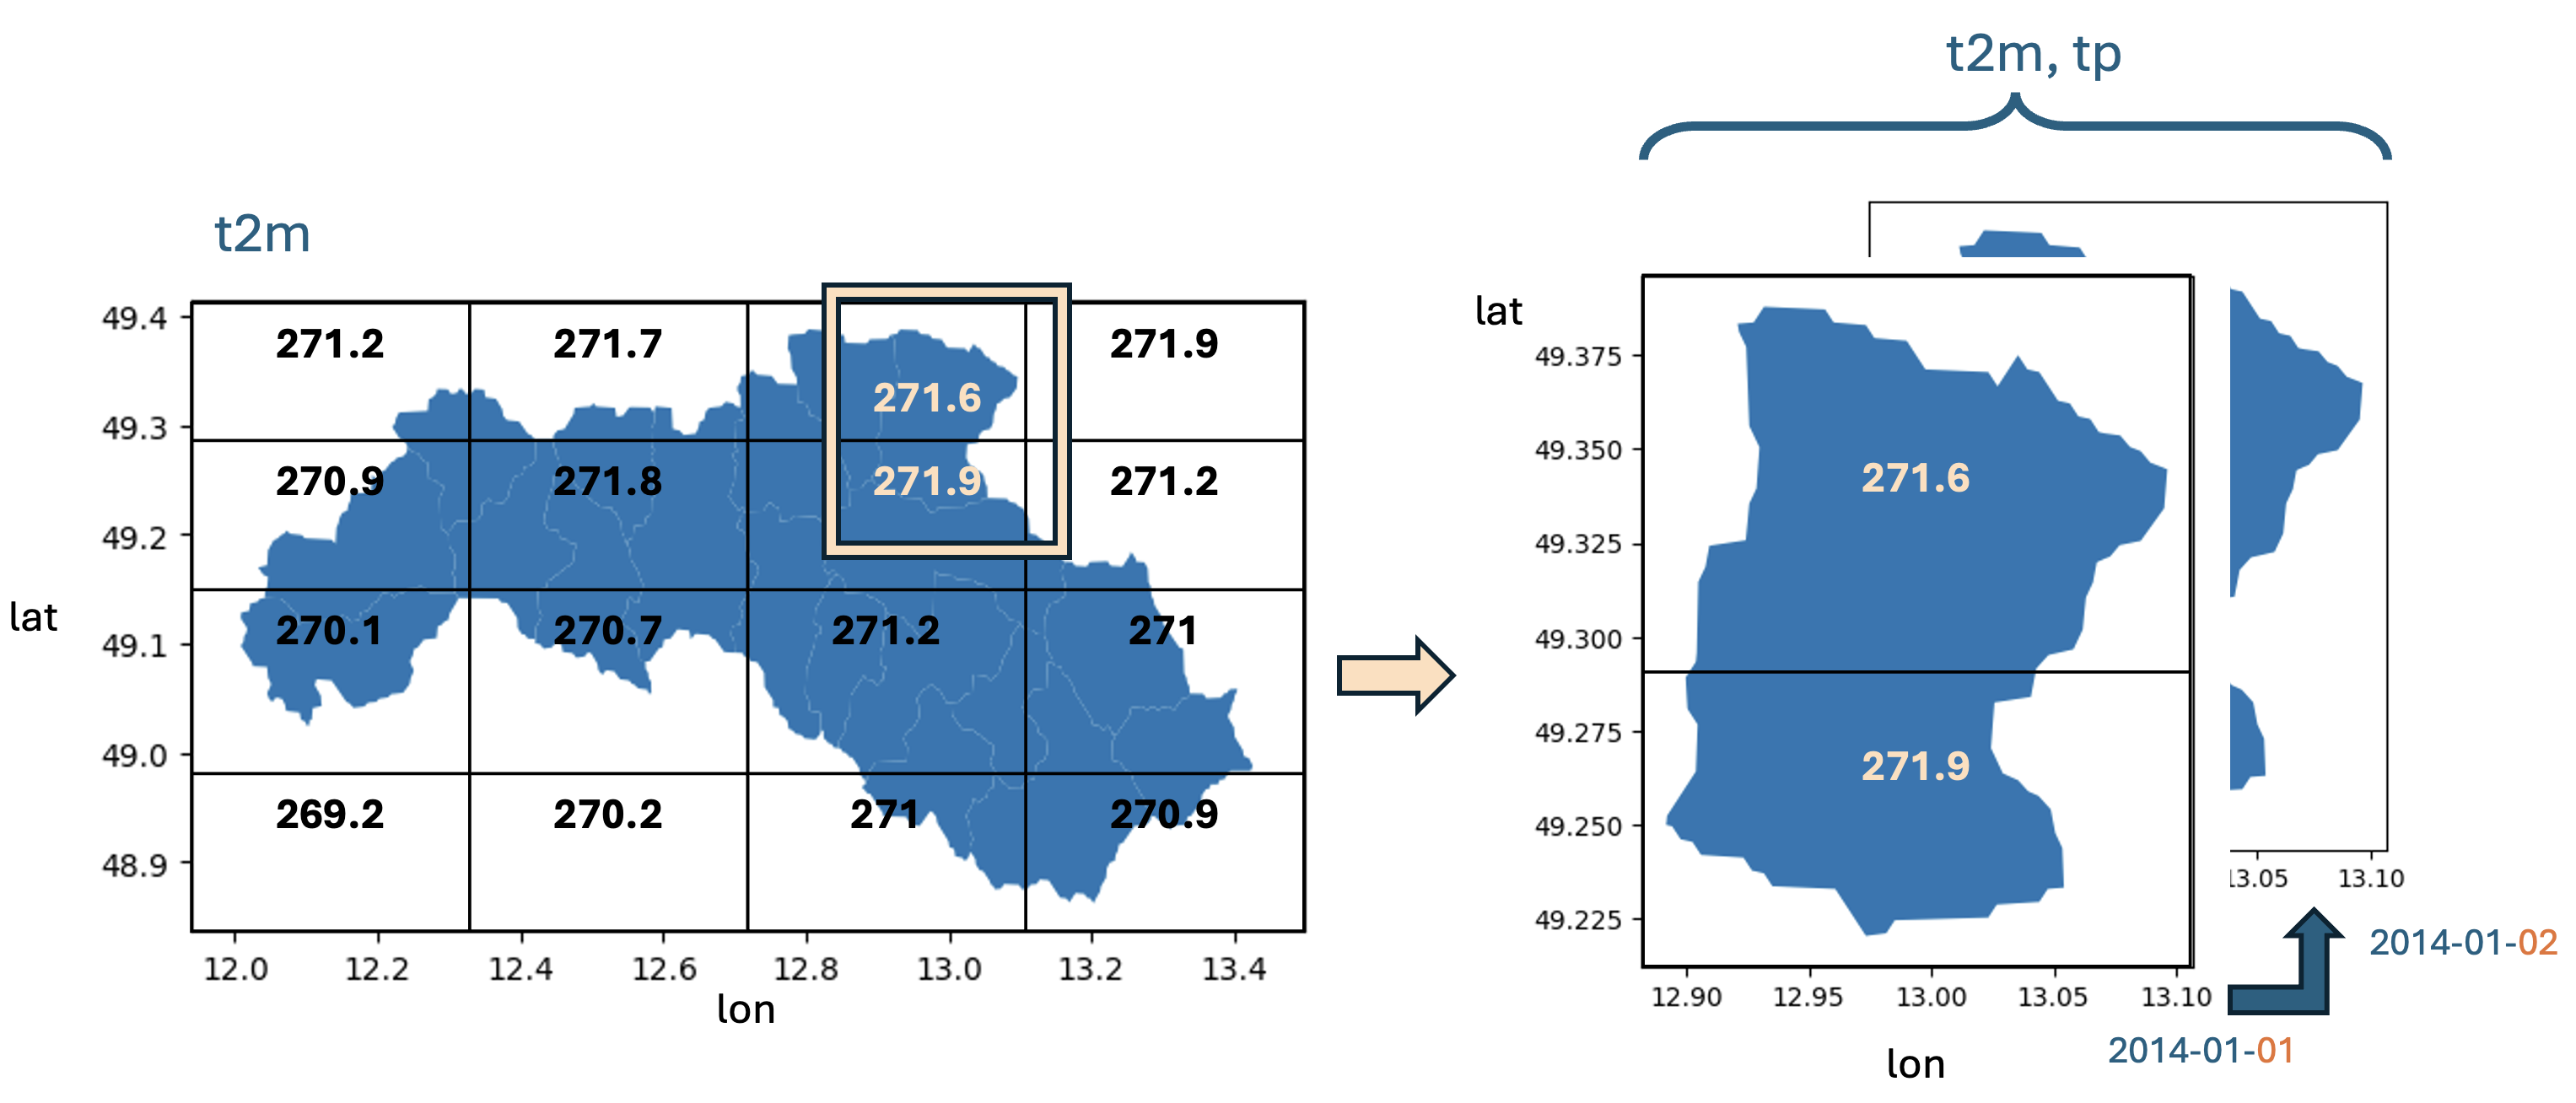
\includegraphics[width=500]{work/07-hydroLSTM/images/spatial_averaging} 

}

\caption{schematic visualization of the spatial averaging performed for temperature and total precipitation during data preprocessing}\label{fig:4}
\end{figure}

\[ t2m(\text{catch}_i) = \frac{1}{A(\text{catch}_i)} \sum_{j \in \text{ERA5 raster}} \left( t2m(\text{cell}_j) \cdot A(\text{catch}_i \cap \text{cell}_j) \right) \tag{1} \]

Since the catchments are geospatially close to each other the different
values in the catchments provided little variance. (IMAGE CORRELATION
Table). To reduce the feature space for both variables temperature and
precipitation, the mean is taken over all catchments. Finally to reduce
the noise in the features a moving average of window size 3 was applied.

\hypertarget{models}{%
\subsection{Models}\label{models}}

\hypertarget{lstm}{%
\subsubsection{LSTM}\label{lstm}}

The Long Short-Term Memory (LSTM) cell (figure @ref(fig:5)) is a type of
recurrent neural network (RNN) architecture designed to model temporal
sequences and their long-range dependencies more accurately than
traditional RNNs. LSTMs were introduced by Sepp Hochreiter and Jürgen
Schmidhuber in 1997 ( Citation missing) to address the issue of
vanishing and exploding gradients encountered in traditional RNNs, which
struggle to maintain context over long sequences.

\begin{figure}

{\centering 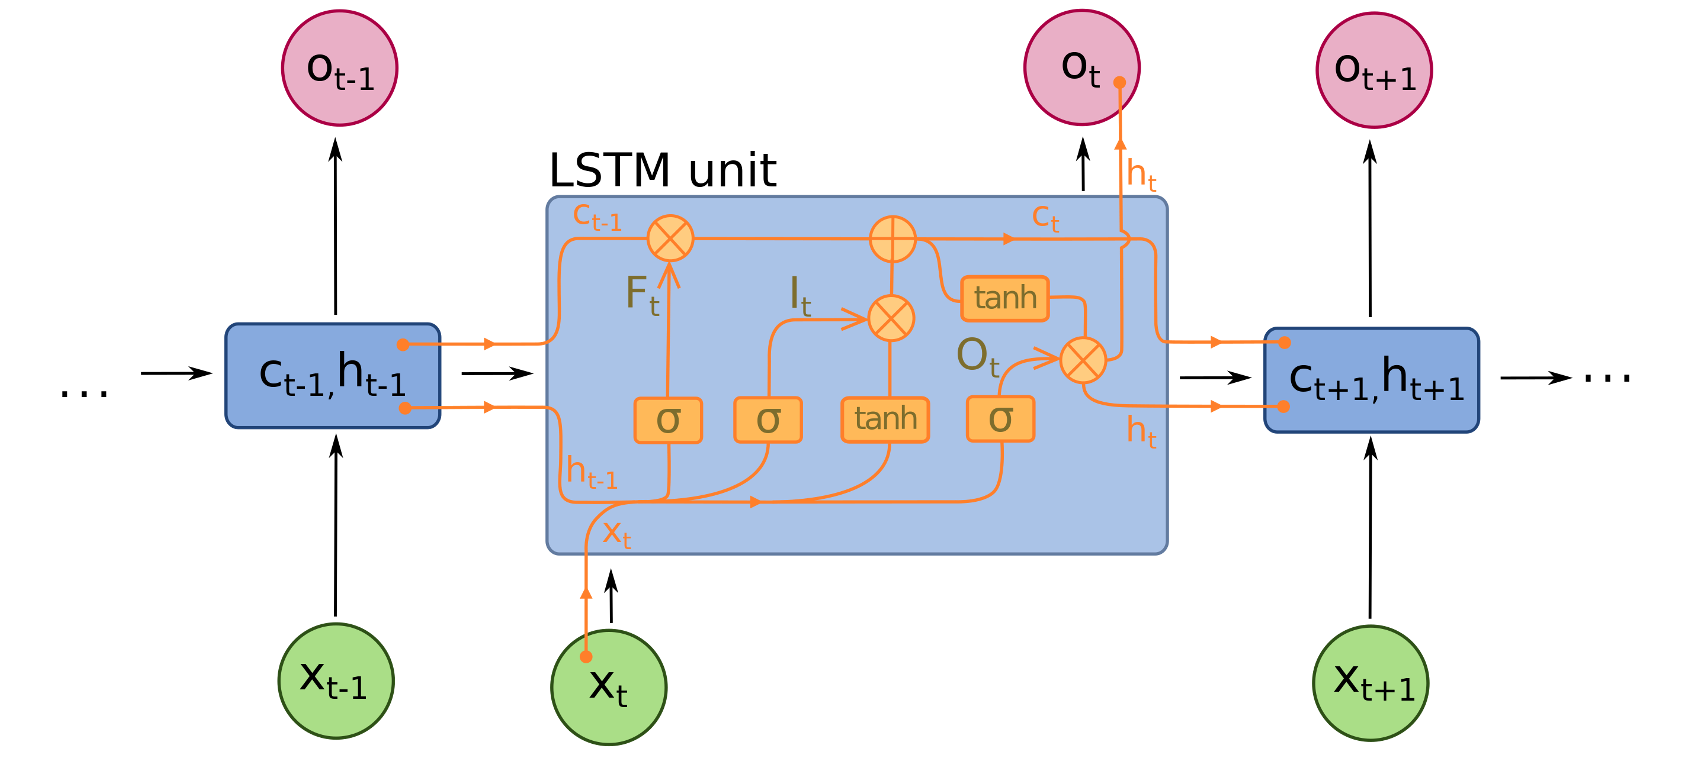
\includegraphics[width=500]{work/07-hydroLSTM/images/LSTM} 

}

\caption{visualization of a LSTM cell at time step t}\label{fig:5}
\end{figure}

\begin{enumerate}
\def\labelenumi{\arabic{enumi}.}
\tightlist
\item
  \textbf{Cell State (}\(C_t\)): The internal memory of the cell, which
  can carry information across many time steps.
\item
  \textbf{Hidden State (}\(h_t\)): The output of the LSTM cell at a
  given time step, also serving as the input to the next cell.
\item
  \textbf{Input Gate (}\(i_t\)): Controls how much of the new
  information from the current input is used to update the cell state.
\item
  \textbf{Forget Gate (}\(f_t\)): Decides how much of the past cell
  state should be forgotten.
\item
  \textbf{Output Gate (}\(o_t\)): Determines the output of the LSTM cell
  based on the cell state.
\end{enumerate}

LSTMs are particularly well-suited for tasks that involve sequential
data and temporal dependencies, such as:

\begin{enumerate}
\def\labelenumi{\arabic{enumi}.}
\tightlist
\item
  \textbf{Natural Language Processing (NLP)}:

  \begin{itemize}
  \tightlist
  \item
    Language modeling
  \item
    Machine translation
  \item
    Speech recognition
  \end{itemize}
\item
  \textbf{Time Series Forecasting}:

  \begin{itemize}
  \tightlist
  \item
    Stock price prediction
  \item
    Weather forecasting
  \item
    Anomaly detection
  \end{itemize}
\end{enumerate}

Streamflow forecasting involves predicting the flow of water in rivers
and streams over time, which is inherently a time-series problem with
temporal dependencies influenced by various factors such as rainfall,
snowmelt, and upstream water management. When used in an encoder decoder
architecture LSTM-cells can also incorporate Future known covariates
such as weather forecasts. These specifications make LSTM-based
architectures beneficial for modeling and forecasting streamflow data.

\hypertarget{temporal-fusion-transformer}{%
\subsubsection{Temporal Fusion
Transformer}\label{temporal-fusion-transformer}}

The Temporal Fusion Transformer (TFT) (figure @ref(fig:6)) is a neural
network architecture specifically designed for multi-horizon time series
forecasting. It combines the strengths of both recurrent and
attention-based models, offering an advanced approach to handling
complex time series data. The TFT was introduced by Bryan Lim et al.~in
2019, aiming to provide interpretability and accuracy for forecasting
tasks.

\begin{figure}

{\centering 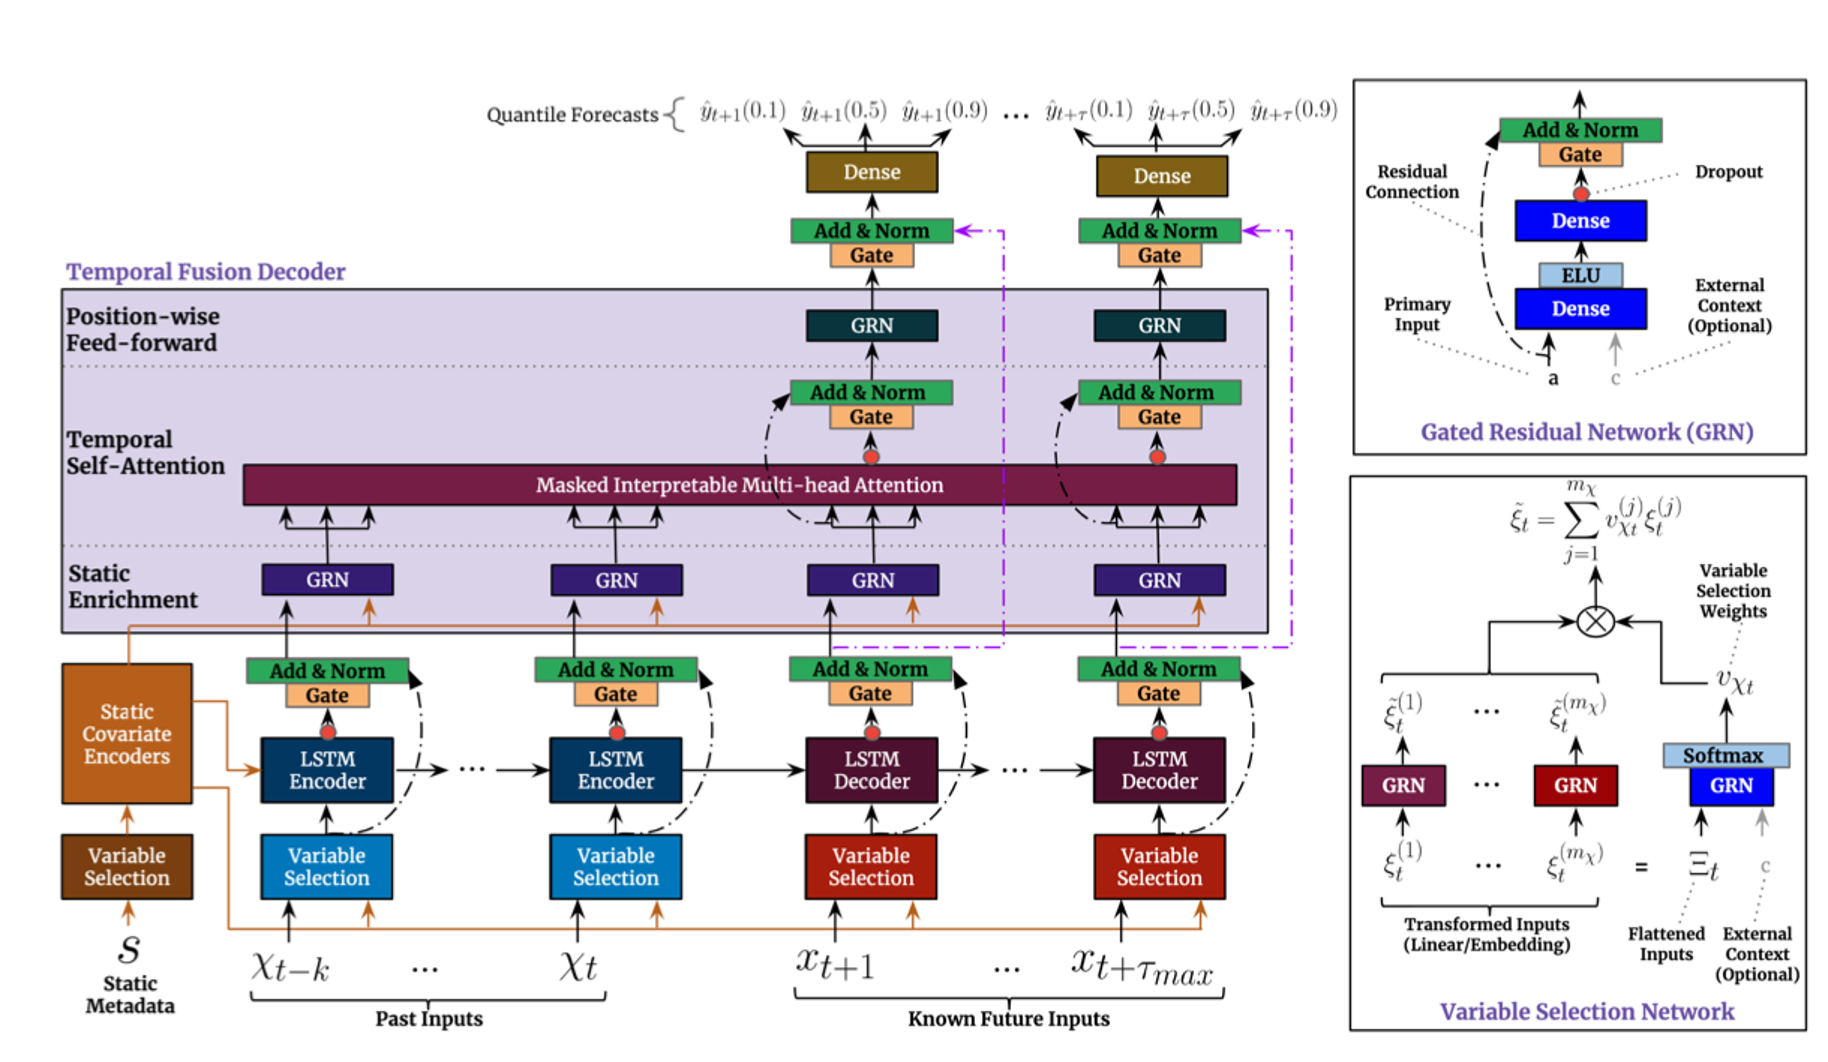
\includegraphics[width=500]{work/07-hydroLSTM/images/TFT} 

}

\caption{model architecture for the Temporal Fusion Transformer}\label{fig:6}
\end{figure}

A TFT consists of several key components:

\begin{enumerate}
\def\labelenumi{\arabic{enumi}.}
\tightlist
\item
  \textbf{Temporal Processing}:

  \begin{itemize}
  \tightlist
  \item
    \textbf{Local Processing with LSTMs}: LSTMs are used to process
    local temporal dependencies within the time series.
  \item
    \textbf{Multi-Head Attention}: An attention mechanism to capture
    long-range dependencies across different time steps.
  \end{itemize}
\item
  \textbf{Variable Selection}:

  \begin{itemize}
  \tightlist
  \item
    \textbf{Static Covariate Encoders}: Handle static features that do
    not change over time (e.g., location-specific data).
  \item
    \textbf{Temporal Covariate Encoders}: Manage time-varying features
    (e.g., weather data, past values of the time series).
  \end{itemize}
\item
  \textbf{Gating Mechanisms}:

  \begin{itemize}
  \tightlist
  \item
    \textbf{Gated Residual Network (GRN)}: Ensures that only relevant
    information is passed through layers, improving the network's
    efficiency and interpretability.
  \item
    \textbf{Variable Selection Networks}: Dynamically select relevant
    variables at each time step to enhance model performance and
    interpretability.
  \end{itemize}
\item
  \textbf{Multi-Horizon Forecasting}:

  \begin{itemize}
  \tightlist
  \item
    \textbf{Sequence-to-Sequence Framework}: Allows the TFT to generate
    forecasts for multiple future time steps simultaneously.
  \end{itemize}
\item
  \textbf{Interpretable Outputs}:

  \begin{itemize}
  \tightlist
  \item
    \textbf{Attention Weights}: Provide insights into which time steps
    and variables the model is focusing on, aiding interpretability.
  \end{itemize}
\end{enumerate}

The Temporal Fusion Transformer represents an advancement in time series
forecasting, offering both high accuracy and interpretability. Its
ability to capture complex dependencies, dynamically select relevant
features, and provide insights into the decision-making process makes it
a useful tool for streamflow forecasting.

\hypertarget{kling-gupta-efficiency}{%
\subsubsection{Kling Gupta Efficiency}\label{kling-gupta-efficiency}}

The Kling-Gupta Efficiency (KGE) is a statistical metric used to
evaluate the performance of hydrological models by comparing simulated
data to observed data. Developed by Gupta et al.~in 2009, the KGE
addresses limitations found in traditional metrics such as the
Nash-Sutcliffe Efficiency (NSE). The KGE decomposes the evaluation of
model performance into three distinct components, providing a more
comprehensive assessment. These components are correlation, bias, and
variability, which help in understanding different aspects of the
model's accuracy.

The KGE is calculated using the following formula:

\[ \text{KGE} = 1 - \sqrt{(r - 1)^2 + (\alpha - 1)^2 + (\beta - 1)^2} \tag{2} \]

\begin{itemize}
\item
  \(r\) is the Pearson correlation coefficient between the simulated and
  observed values.
\item
  \(\alpha\) is the bias ratio, defined as the ratio of the mean of the
  simulated values to the mean of the observed values.
\item
  \(\beta\) is the standard deviation ratio, defined as the ratio of the
  standard deviation of the simulated values to the standard deviation
  of the observed values.
\end{itemize}

\hypertarget{results}{%
\subsection{Results}\label{results}}

\hypertarget{training-setup}{%
\subsubsection{Training Setup}\label{training-setup}}

The 2 different model architectures were trained using the historical
streamflows as well as temperature and precipitation as covariates.
Using an input sequence length of 364 days and an output lead time of up
to 7 days. Temperature and precipitation can be used as future known
values when considering weather forecasts. For example when trying to
predict one step ahead forecast for the streamflow in addition to the
past 364 days of precipitation values one can consider the precipitation
forecast for the next day to get the best predictions possible.

The LSTM Model is run in an encoder decoder architecture, were the past
364 days are the input for an LSTM cell which returns a hidden state and
an output as the encoder step. During the decoder step the encoder
hidden state is fed into the decoder LSTM including the future known
inputs. The model always predicts incrementally in the sense that for
example to predict a 3 step ahead forecast it firsts predicts 1 and 2
step forecast and uses both forecasts to then predict the 3 step
prediction. Both model architectures were used from the
pytorch-forecasting library (SOURCE). The models were retrained for the
different lead times. The used hyperparameters for both models are shown
in Table @ref(tab:tab-1).

\begin{longtable}[]{@{}
  >{\raggedright\arraybackslash}p{(\columnwidth - 4\tabcolsep) * \real{0.4286}}
  >{\raggedright\arraybackslash}p{(\columnwidth - 4\tabcolsep) * \real{0.2857}}
  >{\raggedright\arraybackslash}p{(\columnwidth - 4\tabcolsep) * \real{0.2857}}@{}}
\caption{Hyperparameter comparison between LSTM and TFT.}\tabularnewline
\toprule\noalign{}
\begin{minipage}[b]{\linewidth}\raggedright
Hyperparameter
\end{minipage} & \begin{minipage}[b]{\linewidth}\raggedright
LSTM
\end{minipage} & \begin{minipage}[b]{\linewidth}\raggedright
TFT
\end{minipage} \\
\midrule\noalign{}
\endfirsthead
\toprule\noalign{}
\begin{minipage}[b]{\linewidth}\raggedright
Hyperparameter
\end{minipage} & \begin{minipage}[b]{\linewidth}\raggedright
LSTM
\end{minipage} & \begin{minipage}[b]{\linewidth}\raggedright
TFT
\end{minipage} \\
\midrule\noalign{}
\endhead
\bottomrule\noalign{}
\endlastfoot
Batch Size & 128 & 128 \\
Epochs & 100 & 80 \\
Hidden Size & 128 & 128 \\
Attention Head Size & - & 2 \\
Learning Rate & 0.001 & 0.003 \\
Dropout & 0.2 & 0.1 \\
Weight Decay & 0.001 & 1e-04 \\
Gradient Clipping & 0.1 & 0.1 \\
Loss Function & Mean Absolute Error & Mean Absolute Error \\
Optimizer & Adam & Adam \\
Reduce on Plateau Patience & 7 & 7 \\
Time Varying Known Features & t2m, tp & t2m, tp \\
Time Varying Unknown Features & Streamflow 15207507 & Streamflow
15207507 \\
\end{longtable}

\hypertarget{results-1}{%
\subsubsection{Results}\label{results-1}}

The models show good performance for lead times of 1 and 2 days
especially considering since the training and validation loss that is
used is the MAE and not the KGE. The performance declines sharply for
the LSTM model across the lead times while the decline for the TFT is
more gradual as can be seen in Table @ref(tab:tab-2).

\begin{longtable}[]{@{}rll@{}}
\caption{Performance comparison between TFT and LSTM models across
different lead times. Better performing model for each lead time in
bold}\tabularnewline
\toprule\noalign{}
Lead.Time & TFT.KGE & LSTM.KGE \\
\midrule\noalign{}
\endfirsthead
\toprule\noalign{}
Lead.Time & TFT.KGE & LSTM.KGE \\
\midrule\noalign{}
\endhead
\bottomrule\noalign{}
\endlastfoot
1 & 0.8352 & \textbf{0.9696} \\
2 & 0.7103 & \textbf{0.8821} \\
3 & 0.6410 & \textbf{0.6716} \\
4 & \textbf{0.6096} & 0.4943 \\
5 & \textbf{0.5901} & 0.4302 \\
6 & \textbf{0.5778} & 0.3312 \\
7 & \textbf{0.5717} & 0.3185 \\
\end{longtable}

The forecasting the peaks of the streamflows is especially challenging
and neither model performs particularly well on this task. Especially
when considering that the peaks were drastically reduced due to the
moving average smoothing of the target variable. This behaviour can be
observed on most lead times here shown for a lead time of 5 days for the
LSTM Model and the TFT Model in figure @ref(fig:7) and in figure
@ref(fig:8) respectively.

\begin{figure}

{\centering 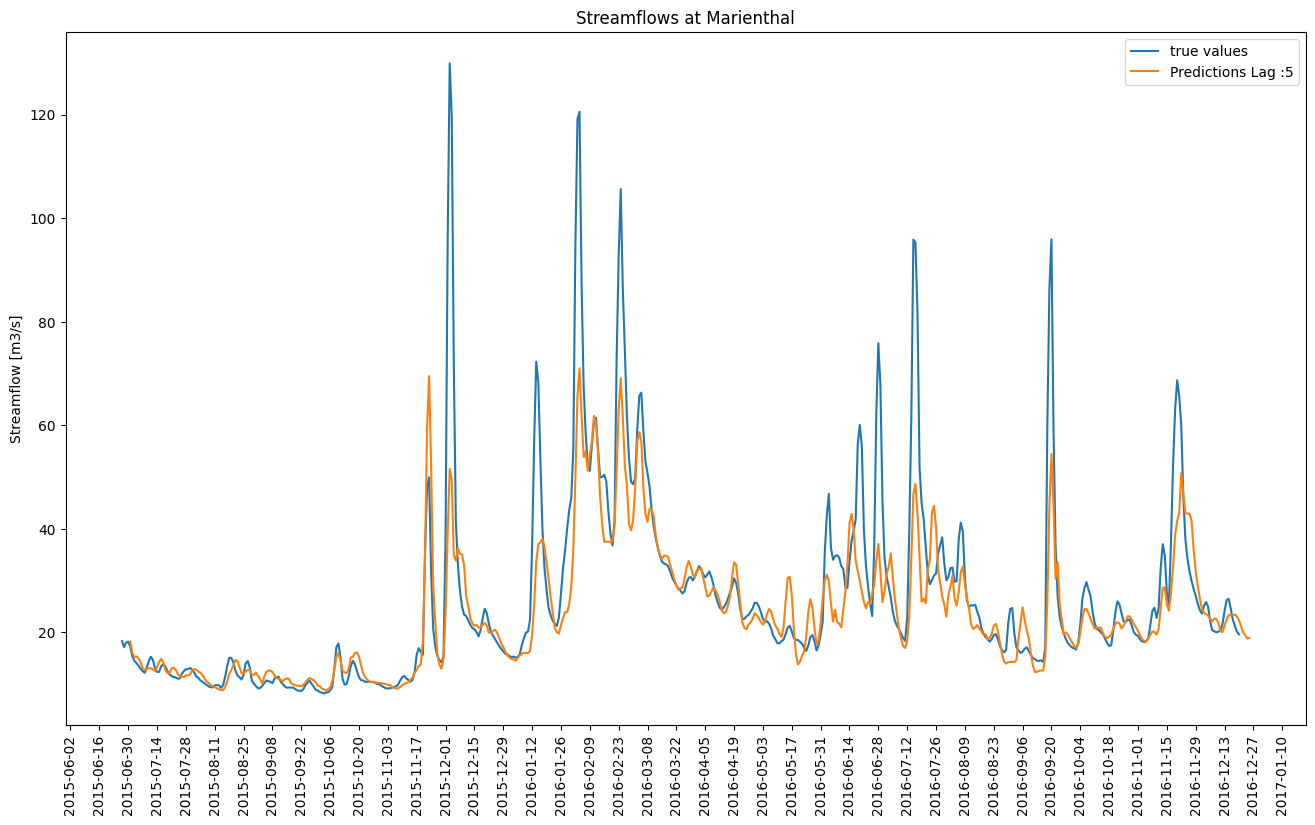
\includegraphics[width=500]{work/07-hydroLSTM/images/lag5_lstm} 

}

\caption{LSTM predicted streamflows for a lead time of 5 days (orange) compared to the observed streamflows (blue)}\label{fig:7}
\end{figure}

\begin{figure}

{\centering 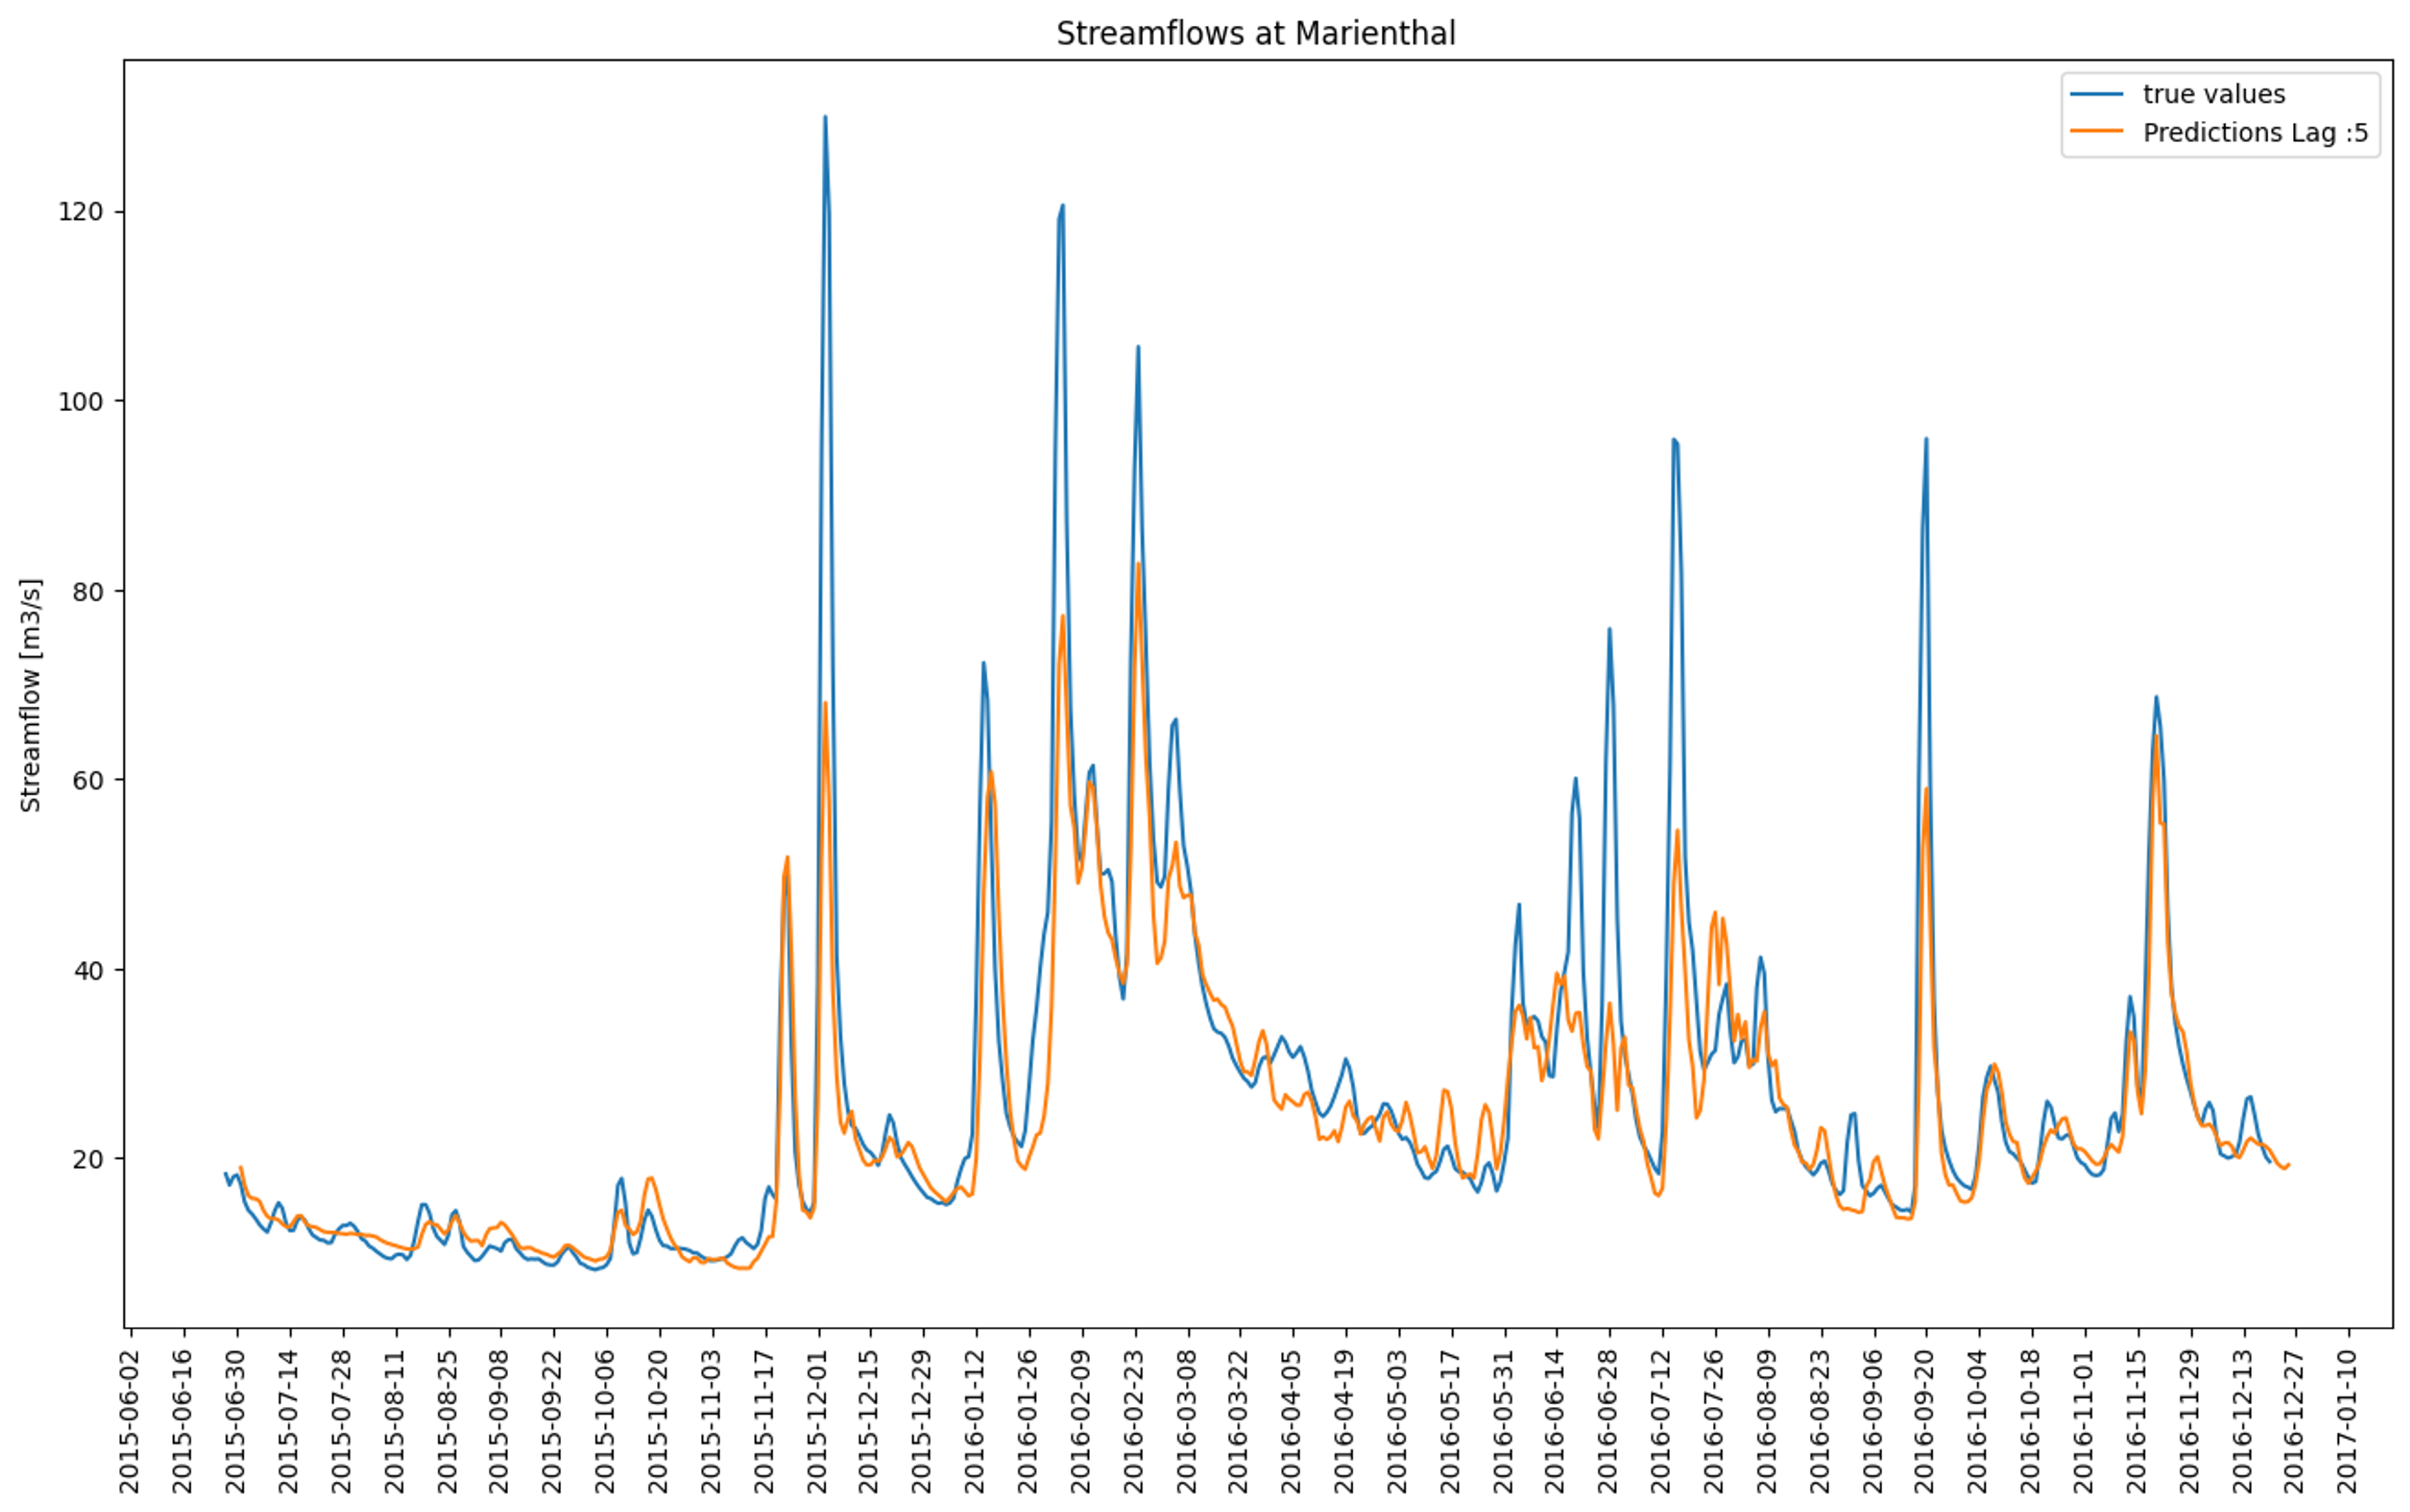
\includegraphics[width=500]{work/07-hydroLSTM/images/lag5_tft} 

}

\caption{TFT predicted streamflows for a lead time of 5 days (orange) compared to the observed streamflows (blue)}\label{fig:8}
\end{figure}

\hypertarget{conclusion}{%
\subsection{Conclusion}\label{conclusion}}

In this study, we compared the performance of LSTM (Long Short-Term
Memory) and Temporal Fusion Transformer (TFT) models in forecasting
streamflows up to seven days ahead, using precipitation and temperature
as future known covariates alongside historical streamflow data.

Our findings indicate that both models exhibit limitations in predicting
extreme values such as floods, with KGE (Kling-Gupta Efficiency) scores
significantly lower than those reported in similar studies, likely due
to reduced data availability and the challenges inherent in modeling a
river system instead of a reservoir. The results also demonstrate a
clear difference in performance trends between the two models across
different lead times.

The LSTM model's KGE scores decline sharply with increasing lead time,
starting at 0.9696 for a one-day lead time and dropping to 0.3185 for a
seven-day lead time. Conversely, the TFT model shows a more gradual
decline, from 0.8352 at one day to 0.5717 at seven days, suggesting it
maintains more consistent accuracy over longer forecast horizons.

Despite the sharper decline in performance for longer lead times, the
LSTM model is notably less resource-dependent, making it a viable option
for scenarios where computational resources are limited. However, our
attempts to forecast streamflows without future known meteorological
variables were unsuccessful, underscoring the importance of these
covariates in achieving accurate predictions.

In summary, while TFT demonstrates better stability over extended
forecast periods, the LSTM model offers advantages in resource
efficiency. Future work should explore strategies to improve model
robustness for extreme value prediction and investigate additional data
sources to enhance forecast accuracy.

\hypertarget{outlook}{%
\subsection{Outlook}\label{outlook}}

Firstly, implementing a robust hyperparameter tuning routine is
essential to optimize model performance. This process will require
additional computational resources due to the complexity and extensive
search space. Given the high dependency of hyperparameters on lag, it is
crucial to carefully adjust them to capture the temporal dynamics
accurately.

Improving data preprocessing is another critical aspect. This includes
downscaling meteorological variables to ensure the input data aligns
better with the spatial and temporal resolution required for accurate
streamflow predictions. Performance optimization techniques will also be
explored to streamline the computational efficiency of the models.

To make the models more sensitive to extreme events such as floods,
specialized training techniques and loss functions will be employed.
Experimentation with different model architectures could offer insights
into more effective structures for capturing the complex patterns in
river streamflow data.

The models need to generalize across different rivers, which involves
accounting for diverse hydrological and geographical characteristics.
Including static variables such as river basin properties and land use
information will help in creating a more comprehensive model that can
adapt to various river systems.

While the moving average is used in (PAPER SOURCE), it is not advised to
use it for streamflow forecasting. By reducing the peaks in the target
variable it artificially boosts the predictive abitlity of the model,
but also forces the model to miss the peaks by an even larger margin. In
a flood scenario even with a high KGE, the model would always miss the
exact streamflow value as it was trained on lower peaks and would
underestimate the posed danger in the situation.

\end{document}
